% Author: Alejandro Santomé Valverde

\chapter{Introduction and thesis objectives} \label{chap:intro}

\section{Integrated photonics} \label{sec:integrated_photonics}

Since the advent of electronic integrated circuits in the second half of the twentieth century, 
the integration of multiple functionalities onto a single chip has been a driving force behind 
the rapid evolution of information and communication technologies 
\cite{mooreCrammingMoreComponents1965a}. The formulation of Moore's law provided a conceptual 
framework that guided the semiconductor industry for decades, enabling an exponential increase in 
transistor density and computational capability. This relentless scaling, together with advances 
in lithography, materials, and fabrication processes, laid the foundation for modern computing, 
signal processing, and digital communication systems.

However, as device dimensions continued to shrink and operating frequencies increased, fundamental 
limitations of electronic integration became increasingly apparent. In particular, issues related 
to bandwidth constraints, power dissipation, latency, and interconnect scalability emerged as major
bottlenecks in advanced electronic systems \cite{millerRationaleChallengesOptical2000}. While 
transistor switching speeds continued to improve, the performance of electrical interconnects 
failed to scale at the same pace, leading to growing energy consumption and thermal management 
challenges \cite{millerDeviceRequirementsOptical2009}. These limitations are especially pronounced 
in large-scale systems, such as data centers and high-performance computing architectures, where 
interconnects dominate both power budgets and system-level performance 
\cite{shalfExascaleComputingTechnology2011}.

In parallel with these developments, photonics emerged as a powerful alternative for signal 
generation, transmission, and processing. The invention of the laser marked a pivotal milestone in 
the field of optics, enabling coherent light sources with unprecedented intensity and spectral 
purity \cite{maimanStimulatedOpticalRadiation1960}. This breakthrough, combined with the 
development of low-loss optical fibers, paved the way for optical communication systems capable of 
transmitting information over long distances with minimal attenuation. Over the following decades, 
photonic technologies became indispensable in global telecommunication infrastructures, 
demonstrating clear advantages over purely electronic approaches in terms of bandwidth and signal 
integrity.

Building upon decades of progress in discrete optical components, integrated photonics arose as a 
natural extension of the integration paradigm pioneered by electronics 
\cite{sorefPresentFutureSilicon2006}. Rather than relying on bulky and alignment-sensitive discrete 
elements, integrated photonics enables the monolithic or hybrid integration of multiple optical 
functions on a single substrate. By bringing together waveguides, modulators, filters, 
multiplexers, and photodetectors within a compact footprint, photonic integrated circuits (PICs) 
allow complex optical systems to be realized in a stable, scalable, and reproducible manner 
\cite{thomsonRoadmapSiliconPhotonics2016}. Furthermore, PICs benefit from wafer-scale 
fabrication processes, offering improved yield, reduced cost per function, and compatibility with 
mature semiconductor manufacturing technologies.

In this context, integrated photonics leverages light as the information carrier, offering 
intrinsic advantages over purely electronic circuits. These include ultra-high data transmission 
rates enabled by optical carrier frequencies, low propagation losses in dielectric waveguides, 
immunity to electromagnetic interference, and the ability to support dense wavelength-division 
multiplexing. From an energy perspective, photonic interconnects can significantly reduce power 
consumption by mitigating resistive losses and capacitive charging effects that plague electrical 
interconnects, particularly at high data rates 
\cite{millerRationaleChallengesOptical2000,millerDeviceRequirementsOptical2009}. As electrical 
interconnects increasingly constitute a dominant performance and energy bottleneck, photonic 
solutions have gained substantial interest as a complementary or alternative technology.

As a result, integrated photonics has become a key enabling technology for next-generation 
communication, sensing, and computing systems. Its impact spans a wide range of applications, 
including optical transceivers for data centers, chip-to-chip and on-chip interconnects for 
high-performance computing, microwave photonics, and emerging photonic information processing 
platforms. More recently, the convergence of electronic and photonic integration has given rise to 
heterogeneous and co-integrated systems, where electronic control and photonic signal processing 
are combined to exploit the strengths of both domains 
\cite{youngOpticalTechnologyTeraScale2010,jalaliSiliconPhotonics2006}. 
This convergence positions integrated photonics as a central technology in addressing the 
scalability, performance, and energy-efficiency challenges of future information processing systems 
\cite{bogaertsProgrammablePhotonicCircuits2020}.


\begin{figure}[htbp]
	\begin{center}
		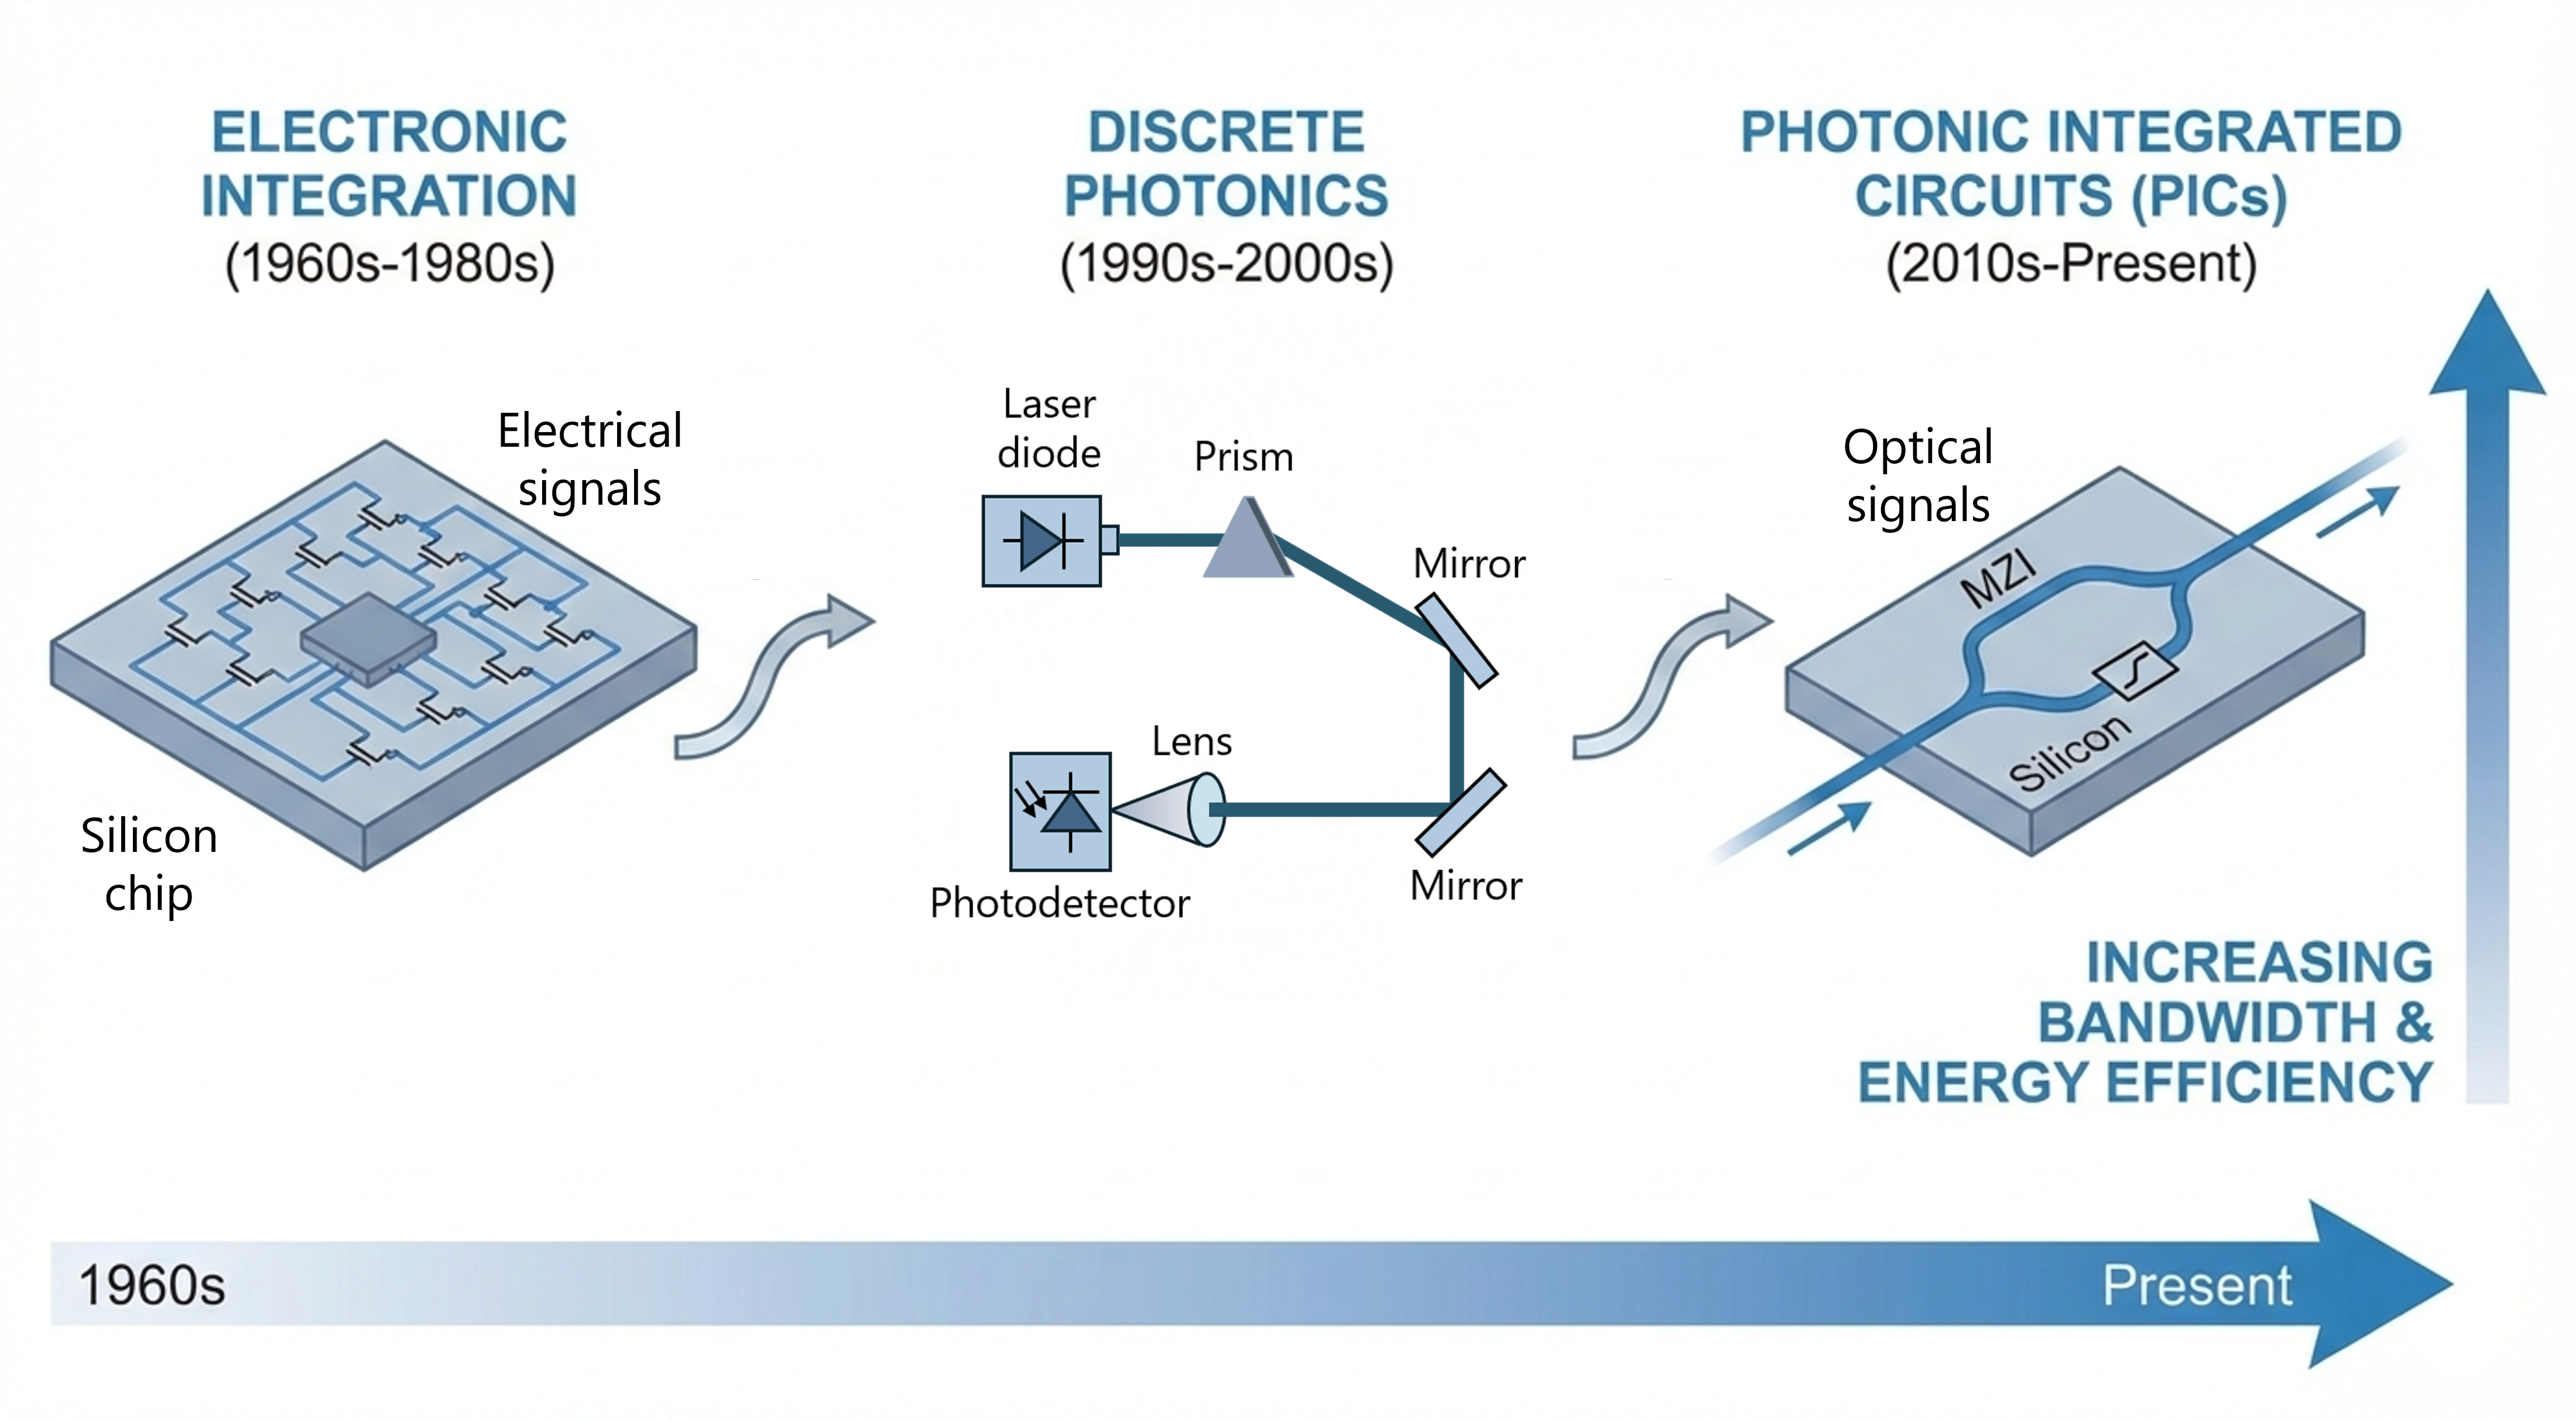
\includegraphics[width=1.0\textwidth]{figures/ch1-evolution.png}
	\end{center}
	\caption{Conceptual evolution from electronic integration to photonic integrated circuits.}\label{fig:ch1-evolution}
\end{figure}




\section{From Application-Specific to Programmable Photonic Integrated Circuits} \label{sec:photonics_motivation}

Early generations of photonic integrated circuits were predominantly designed following an 
application-specific paradigm. In this approach, each PIC was optimized to perform a well-defined 
function, such as optical modulation, filtering, switching, or wavelength multiplexing, with its 
architecture and component parameters tailored to a particular use case. This design philosophy 
enabled highly efficient and compact solutions, and played a crucial role in the successful 
deployment of integrated photonics in applications such as optical communications, sensing, and 
signal processing 
\cite{sorefPresentFutureSilicon2006,liangRecentProgressLasers2010,thomsonRoadmapSiliconPhotonics2016}.

However, as photonic systems grew in complexity and diversity, the shortcomings of purely 
application-specific photonic integrated circuits became increasingly evident. Designing a new PIC 
for each target functionality entails long development cycles, high non-recurring engineering 
costs, and limited flexibility to adapt to evolving system requirements. Moreover, fabrication 
tolerances, environmental fluctuations, and device aging introduce unavoidable variations that can 
significantly degrade the performance of fixed-function photonic circuits if no post-fabrication 
tuning is available \cite{annoniAutomatedRoutingControl2016}.

To mitigate these issues, reconfigurability was gradually introduced into integrated photonic 
platforms. Initially, tunable elements such as thermo-optic or electro-optic phase shifters were 
incorporated to compensate for fabrication-induced deviations and to enable limited 
post-fabrication trimming. While this represented an important step forward, these early 
reconfigurable circuits were still largely application-specific, as their overall topology and 
functional scope remained fixed at the design stage.

Inspired by the success of programmable electronic hardware and field-programmable gate arrays 
(FPGAs), the concept of programmable photonic integrated circuits emerged as a promising 
alternative to conventional design methodologies \cite{bogaertsProgrammablePhotonicCircuits2020}. 
Rather than implementing a single predefined function, programmable PICs rely on a generic 
hardware architecture that can be configured through software to realize a wide range of photonic 
signal processing tasks. This paradigm shift enables the reuse of the same physical chip across 
multiple applications, significantly reducing development time and cost while increasing 
versatility.

A widely adopted approach to programmable photonics is based on networks of tunable 2x2 
interferometric building blocks, typically implemented as Mach-Zehnder interferometers (MZIs) 
equipped with phase shifters and tunable couplers 
\cite{reckExperimentalRealizationAny1994,perezMultipurposeSiliconPhotonics2017}. By 
appropriately programming theinternal phases and coupling ratios, such meshes can be configured to 
implement arbitrary linear transformations, including filters, switches, beamformers, and mode 
converters. Several mesh topologies have been proposed, including triangular, rectangular, and 
hexagonal arrangements, each offering different trade-offs in terms of scalability, robustness, and 
control complexity \cite{clementsOptimalDesignUniversal2016,perezMultipurposeSiliconPhotonics2017}.

\begin{figure}[htbp]
	\begin{center}
		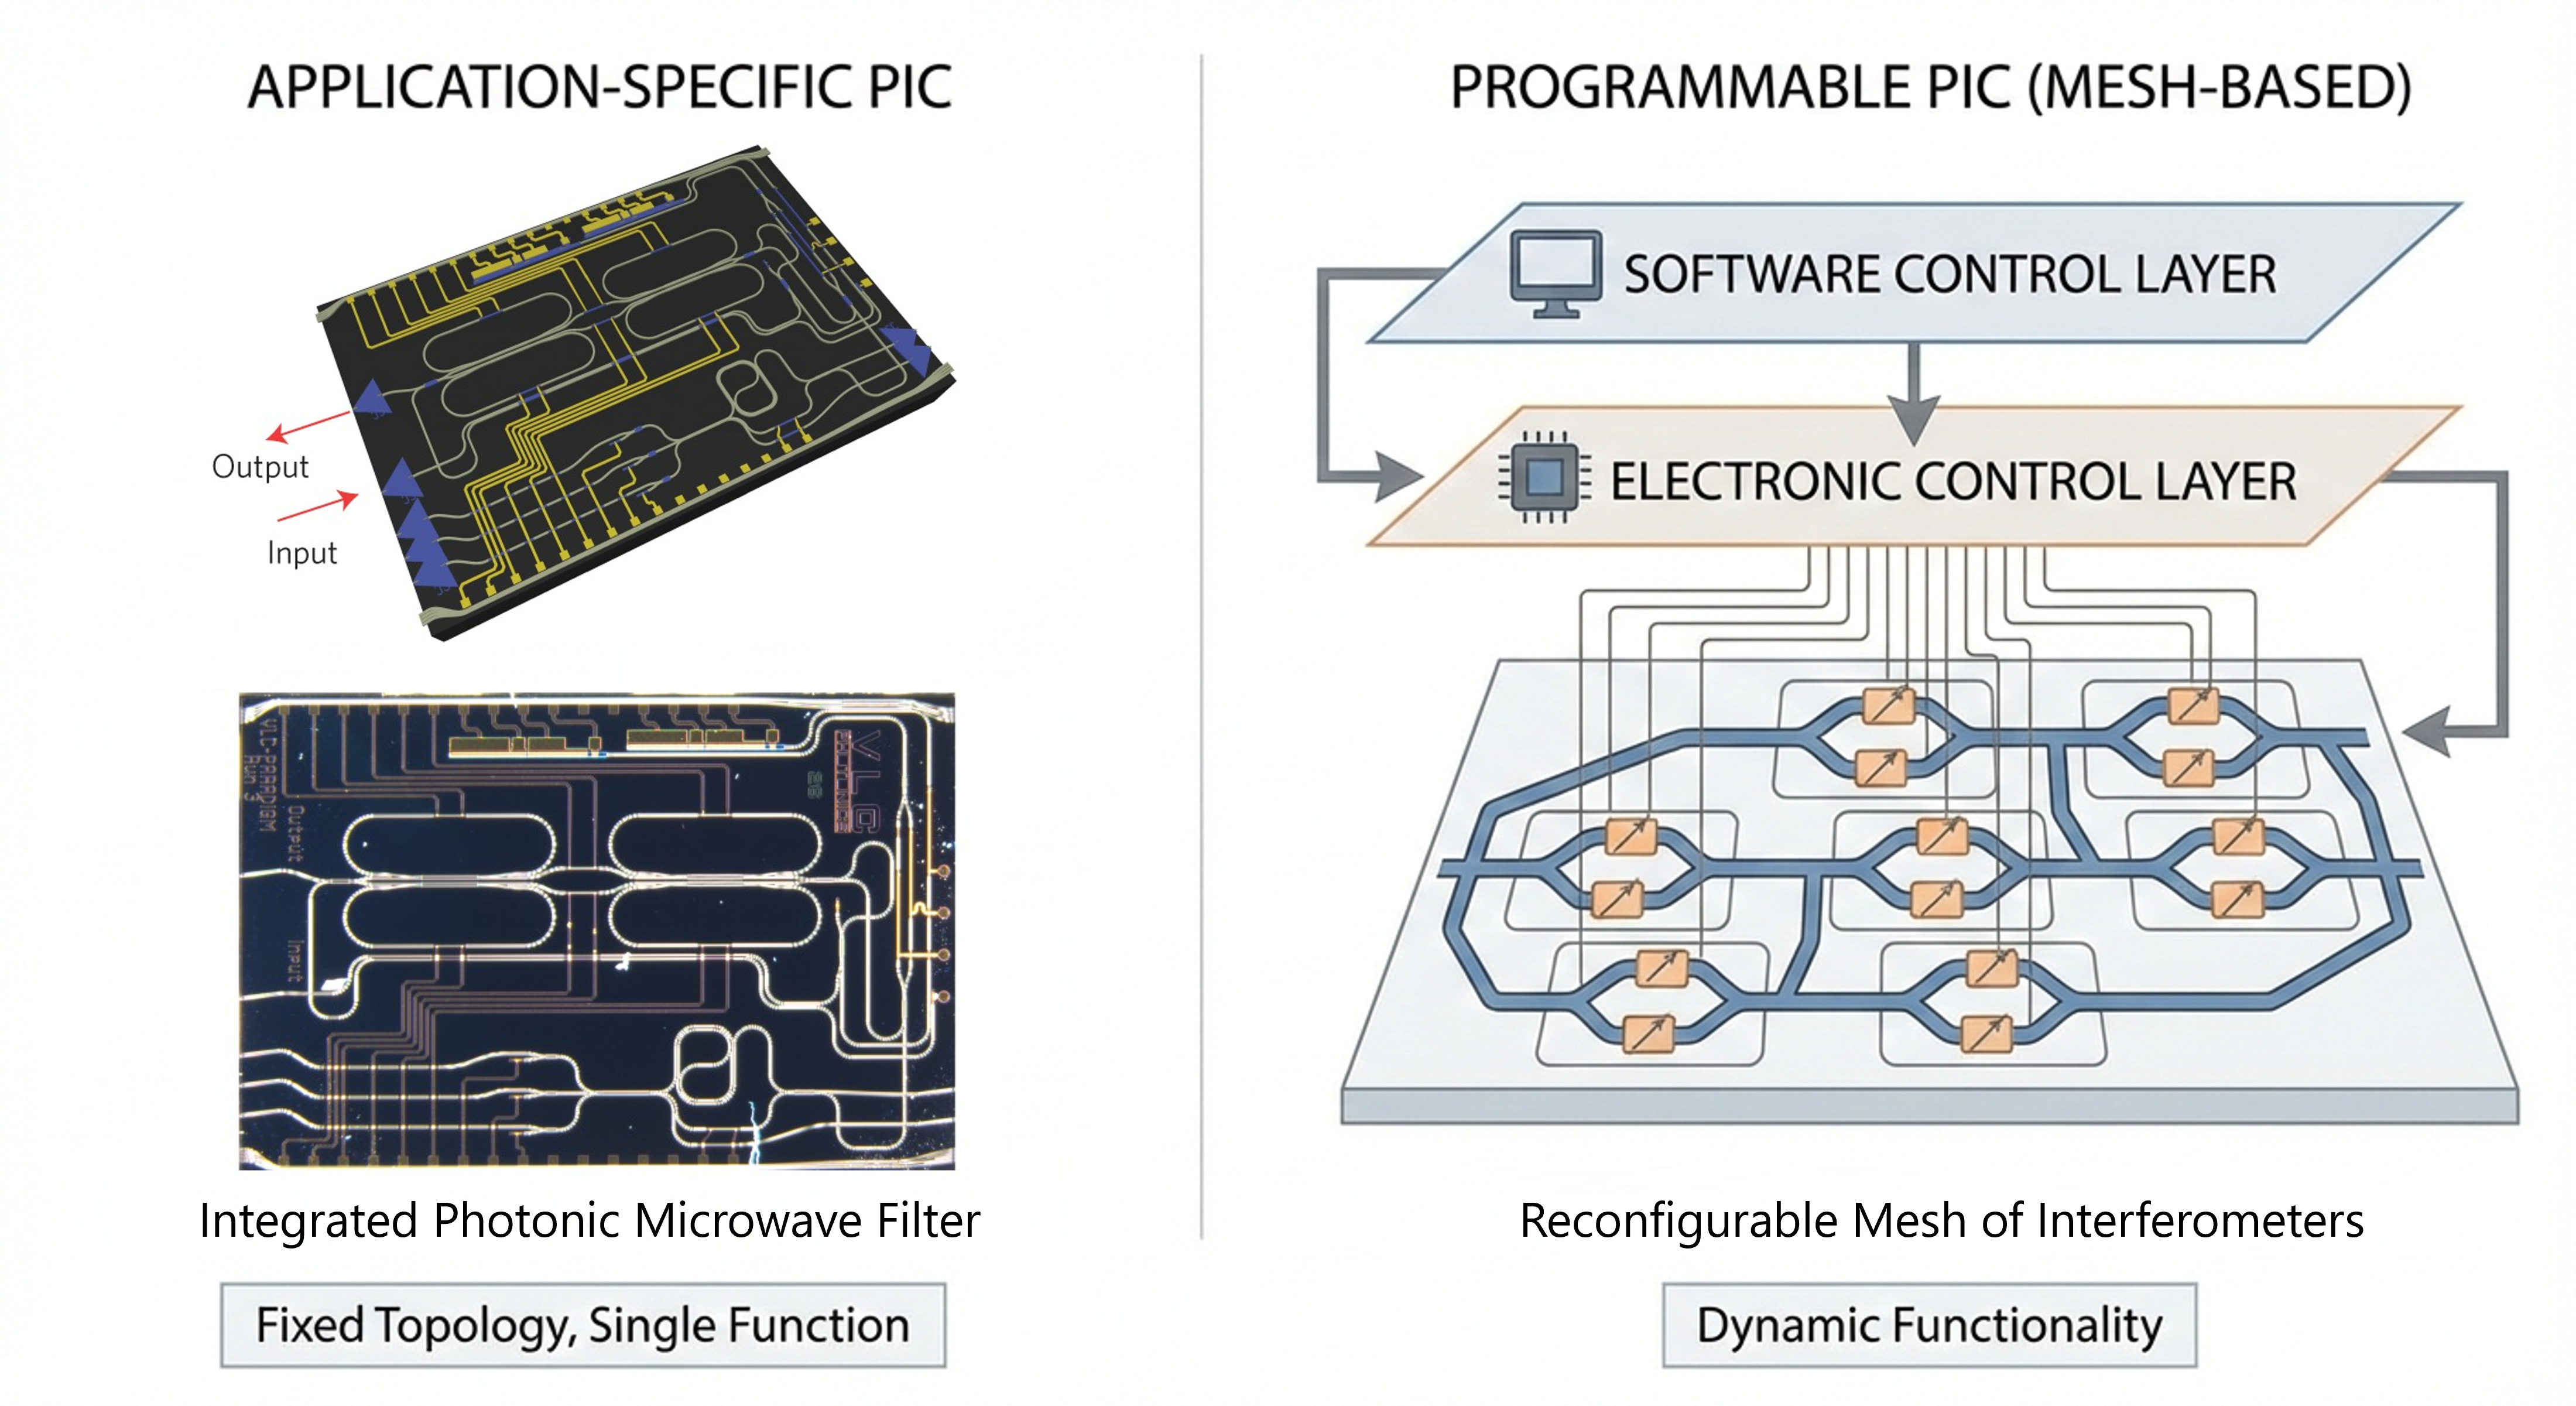
\includegraphics[width=1.0\textwidth]{figures/ch1-aspic_vs_programmable.png}
	\end{center}
	\caption{Application specific PICs versus Programmable PICs.}\label{fig:ch1-aspic_vs_programmable}
\end{figure}

Programmable photonic integrated circuits have demonstrated significant potential in a broad range 
of applications. In optical communications, they enable adaptive filtering, dynamic wavelength 
routing, and coherent signal processing \cite{perezReconfigurableLatticeMesh2016}.
% ,perezFieldProgrammablePhotonicArrays2018,lopezProgrammableTrueTime2018
In microwave photonics, programmable PICs provide flexible platforms for beamforming and signal 
generation. More recently, they have attracted considerable attention in emerging areas such as 
optical computing, machine learning, and quantum information processing, where hardware 
adaptability is a critical requirement \cite{shenDeepLearningCoherent2017}.

Despite their promise, programmable photonic integrated circuits also introduce new challenges. 
The large number of tunable elements required for complex meshes leads to increased power 
consumption, control overhead, and calibration complexity. Thermal crosstalk, control drift, and 
scaling limitations must be carefully addressed to ensure stable and reliable operation 
\cite{millerSelfconfiguringUniversalLinear2013,sacchiIntegratedElectronicController2025}. These 
challenges have motivated ongoing research into alternative tuning mechanisms, advanced control 
algorithms, and hybrid electronic-photonic control architectures.

Overall, the transition from application-specific to programmable photonic integrated circuits 
represents a fundamental evolution in the design philosophy of integrated photonics. By decoupling 
hardware from functionality, programmable PICs offer a flexible and scalable platform capable of 
addressing the growing demands of future communication, sensing, and computing systems, while 
accelerating innovation and reducing barriers to entry in photonic system design
\cite{bogaertsProgrammablePhotonicCircuits2020}.
% perezReconfigurablePhotonicProcessors2018




\section{Objectives} \label{sec:objectives}

The overarching objective of this doctoral thesis is to address the scalability challenges of 
programmable photonic integrated circuits, with the aim of enabling their reliable deployment in 
complex, large-scale photonic systems. While programmable PICs offer unprecedented flexibility and 
functional versatility, their practical adoption is currently constrained by limitations related to 
scalability, reliability, fabrication variability, and system-level integration. This work seeks to 
tackle these challenges through a combination of circuit design, architectural strategies, and 
experimental validation.

A first major objective of this thesis is to improve the scalability of programmable PICs in terms 
of the number of tunable elements that can be integrated on a single chip. As programmable photonic 
architectures grow in size and complexity, the cumulative impact of component imperfections, tuning 
errors, and environmental perturbations becomes increasingly critical. Ensuring reliable operation 
in the presence of a large number of active elements requires the development of design 
methodologies and control strategies that enhance robustness and long-term stability. In this 
context, particular emphasis is placed on reliability, understood as the ability of the circuit to 
maintain its intended functionality over time and under realistic operating conditions.

Closely related to this objective is the need to increase fabrication tolerance in programmable 
photonic designs. Variations arising from lithographic inaccuracies, material non-uniformities, and 
process fluctuations are unavoidable in large-scale fabrication. This thesis aims to explore design 
approaches and circuit architectures that are inherently more resilient to such variations, 
reducing sensitivity to fabrication errors and easing post-fabrication calibration and tuning 
requirements. Enhancing fabrication tolerance is a key enabler for scaling programmable PICs beyond 
laboratory demonstrations toward manufacturable and repeatable platforms.

A second central objective is to address scalability at the architectural and system levels. This 
includes the efficient use of on-chip area as programmable meshes increase in size, as well as the 
challenges associated with electrical and optical packaging. As the number of control signals, 
heaters, phase shifters, and optical ports grows, packaging constraints can become a dominant 
bottleneck, affecting power consumption, thermal management, signal integrity, and overall system 
complexity. This thesis seeks to investigate architectural solutions and integration strategies 
that mitigate these constraints, facilitating the realization of scalable programmable photonic 
systems compatible with realistic packaging and interconnection technologies.

Finally, a key objective of this work is to demonstrate the practical applicability of scalable 
programmable PICs through representative use cases and applications. Beyond architectural and 
technological advances, it is essential to show that the proposed scalable solutions can 
effectively support meaningful photonic functionalities. To this end, the thesis aims to validate 
the developed concepts through experimental demonstrations in relevant application scenarios, 
highlighting the benefits of scalability, robustness, and programmability in real-world contexts.

Overall, by addressing scalability across device, circuit, architectural, and application 
dimensions, this thesis aims to contribute to the maturation of programmable photonic integrated 
circuits from flexible research platforms toward reliable and scalable technologies suitable for 
next-generation photonic systems.

% section Objective (end)



\section{Structure of the thesis} \label{sec:structure} 
This manuscript presents the work conducted to obtain the degree of Doctor of Philosophy (PhD) in 
Telecommunication Engineering within the doctoral program of the Universitàt Politècnica de 
València (UPV).

\begin{itemize}
	\item Chapter 1: \nameref{chap:intro}  sets the technological context and research motivation 
		for scalable programmable photonic integrated circuits. It examines the evolution from 
		application-specific PICs to programmable architectures and identifies the key scalability 
		challenges at device, circuit, and system levels. The objectives and scope of the thesis 
		are subsequently defined.
	\item Chapter 2: \nameref{chap:fundamentals}  develops the theoretical and technological 
		framework underlying programmable photonic integrated circuits. It details the operating 
		principles of integrated waveguides and the silicon-on-insulator platform, and examines 
		the passive and active elements forming programmable circuits. The chapter then addresses 
		mesh architectures, sources of scalability degradation, and existing calibration and 
		fault-tolerance techniques for large-scale programmable systems.
		
	\item Chapter 3: 
	
	\item Chapter 4: 

	\item Chapter 5: 
	
\end{itemize}


% At the end of the manuscript, a section is provided with a complete list of the Author’s merits 
% and contributions to scientific journals and conferences.
